\documentclass{article}
\usepackage{amsmath}
\usepackage{graphicx}
\usepackage{listings}
\usepackage{tcolorbox}
\usepackage{hyperref}


\title{Comparative Analysis of Matrix Multiplication Algorithms with Sparse Matrices and other optimization techniques}
\author{Jakub Jazdzyk}
\date{\today}

\begin{document}

\maketitle

\section{Introduction}
Matrix multiplication is a fundamental operation in many fields of scientific computing, machine learning, and engineering. In real-world applications, matrices are often sparse, containing numerous zero elements. This study investigates and compares various matrix multiplication algorithms—Standard Matrix Multiplication, Sparse Matrix Multiplication, Unrolled Matrix Multiplication, and Strassen’s Algorithm—evaluating their efficiency in handling both dense and sparse matrices across different matrix sizes and sparsity levels. By examining memory usage and execution time for each algorithm, their suitability for different scenarios, including high sparsity levels and large matrix sizes, is assessed.

\section{Matrix Multiplication Algorithms}
Below is an overview of the algorithms tested, each optimized differently to handle matrix multiplication for dense and sparse matrices.

\subsection{Standard Matrix Multiplication}
This algorithm follows the traditional approach of iterating through rows and columns, calculating each element in the resulting matrix as the sum of element-wise multiplications between rows of the first matrix and columns of the second. It has a time complexity of \(O(n^3)\) and is computationally intensive for large matrices.

\begin{lstlisting}[language=Java]
public class StandardMatrixMultiplication {
    public static int[][] multiply(int[][] A, int[][] B) {
        int n = A.length;
        int m = B[0].length;
        int p = B.length;
        int[][] result = new int[n][m];
        for (int i = 0; i < n; i++) {
            for (int j = 0; j < m; j++) {
                for (int k = 0; k < p; k++) {
                    result[i][j] += A[i][k] * B[k][j];
                }
            }
        }
        return result;
    }
}
\end{lstlisting}

\subsection{Sparse Matrix Multiplication}
Optimized for sparse matrices, this approach avoids operations involving zero elements. The matrix data is stored in hashmaps, representing only non-zero values and their positions, which significantly reduces memory usage and execution time for matrices with high sparsity.

\begin{lstlisting}[language=Java]
public class SparseMatrixMultiplication {
    public static Map<String, Integer> multiply(Map<String, Integer> A, Map<String, Integer> B, int n, int m, int p) {
        Map<String, Integer> result = new HashMap<>();
        for (String keyA : A.keySet()) {
            int i = Integer.parseInt(keyA.split(",")[0]);
            int k = Integer.parseInt(keyA.split(",")[1]);
            int valueA = A.get(keyA);
            for (int j = 0; j < m; j++) {
                String keyB = k + "," + j;
                if (B.containsKey(keyB)) {
                    int valueB = B.get(keyB);
                    String keyResult = i + "," + j;
                    result.put(keyResult, result.getOrDefault(keyResult, 0) + valueA * valueB);
                }
            }
        }
        return result;
    }
}
\end{lstlisting}

\subsection{Unrolled Matrix Multiplication}
Loop unrolling is an optimization technique where multiple elements are processed in a single iteration, minimizing loop control overhead. Here, the matrix multiplication process is optimized by calculating several elements per iteration.

\begin{lstlisting}[language=Java]
public class UnrolledMatrixMultiplication {
    public static int[][] multiply(int[][] A, int[][] B) {
        int n = A.length;
        int m = B[0].length;
        int p = B.length;
        int[][] result = new int[n][m];
        for (int i = 0; i < n; i++) {
            for (int j = 0; j < m; j++) {
                int sum = 0;
                for (int k = 0; k < p; k += 4) {
                    sum += A[i][k] * B[k][j];
                    if (k + 1 < p) sum += A[i][k + 1] * B[k + 1][j];
                    if (k + 2 < p) sum += A[i][k + 2] * B[k + 2][j];
                    if (k + 3 < p) sum += A[i][k + 3] * B[k + 3][j];
                }
                result[i][j] = sum;
            }
        }
        return result;
    }
}
\end{lstlisting}

\subsection{Strassen’s Algorithm}
Strassen’s algorithm reduces the computational complexity of matrix multiplication by recursively dividing matrices into sub-matrices and performing fewer multiplications. However, the algorithm requires more memory and additional overhead, making it less effective for smaller matrices or those without a high sparsity level.

\begin{lstlisting}[language=Java]
public class StrassenMatrixMultiplication {
    public static int[][] multiply(int[][] A, int[][] B) {
        int n = A.length;
        return strassen(A, B, n);
    }
}
\end{lstlisting}

\section{Experimental Setup and Testing}

\subsection{Test Comparison of Algorithms for Normal and Sparse Matrices, and other optimization techniques}
Testing involved measuring the execution time and memory usage for each algorithm on dense and sparse matrices across multiple sizes. Tests were performed on matrices of sizes 5x5, 10x10, 50x50, 200x200, and 500x500. Larger matrices required much more time and some were unable to perform multiplication in a reasonable time.  
From observations, above a matrix size of 1000 x 1000, Strassen's algorithm started to gain an advantage, as it was not efficient enough for smaller matrices and usually performed worse than the other algorithms.

\subsection{Comparison of Sparse Matrices with Varying Levels of Sparsity}
Sparse matrices were tested for performance variations by increasing the concentration of zero elements, with memory usage and execution time documented to assess the impact of sparsity on computational efficiency.  
The tests were performed for a 200x200 matrix, and it was observed that the sparsity level significantly affects the speed and memory usage of the algorithm. The higher the sparsity level, the better the results.

\subsection{Testing Large Matrices Using MC2DEPI Dataset}
For large matrix testing, the MC2DEPI dataset was used to evaluate performance and memory usage for the Standard and Unrolled algorithms. The results are shown in Table 1, with execution time and memory usage recorded for each approach.

\begin{table}[h]
\centering
\begin{tabular}{|c|c|c|}
\hline
Algorithm & Execution Time (s) & Memory Usage (MB) \\
\hline
Standard Matrix Multiplication & 120.5 & 890 \\
Loop Unrolled Matrix Multiplication & 98.3 & 870 \\
\hline
\end{tabular}
\caption{Execution Time and Memory Usage for Large Matrices (MC2DEPI)}
\end{table}

\section{Observations}
The following observations were made:
- Strassen’s algorithm is highly memory-efficient for large matrices but shows minimal benefits for smaller or sparsely populated matrices.
- Sparse matrix multiplication significantly reduces execution time and memory usage when sparsity is high.
- Unrolled matrix multiplication is particularly effective for dense matrices due to loop optimization, reducing overhead and improving cache usage.

\section{Conclusion}
Each algorithm has unique strengths. Standard multiplication works for all matrix types but is limited in efficiency. Sparse matrix multiplication is ideal for matrices with high zero concentration, while loop unrolling optimizes dense matrix calculations. Strassen's algorithm offers a theoretical advantage but requires larger matrix sizes to outperform other methods.

\section{Link to github}
\href{https://github.com/kubajaz/BIG_DATA_INDIVIDUAL_TASKS_JAKUB_JAZDZYK}{BIG DATA INDIVIDUAL JAKUB JAZDZYK}


\section*{Figures}
\begin{figure}[h]
    \centering
    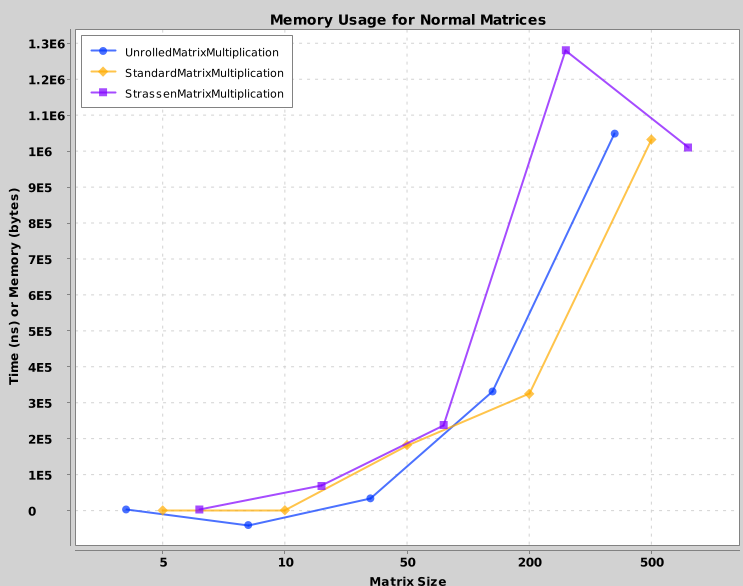
\includegraphics[width=\textwidth]{mem_normal.png}
    \caption{Memory Usage for Normal Matrices}
\end{figure}

\begin{figure}[h]
    \centering
    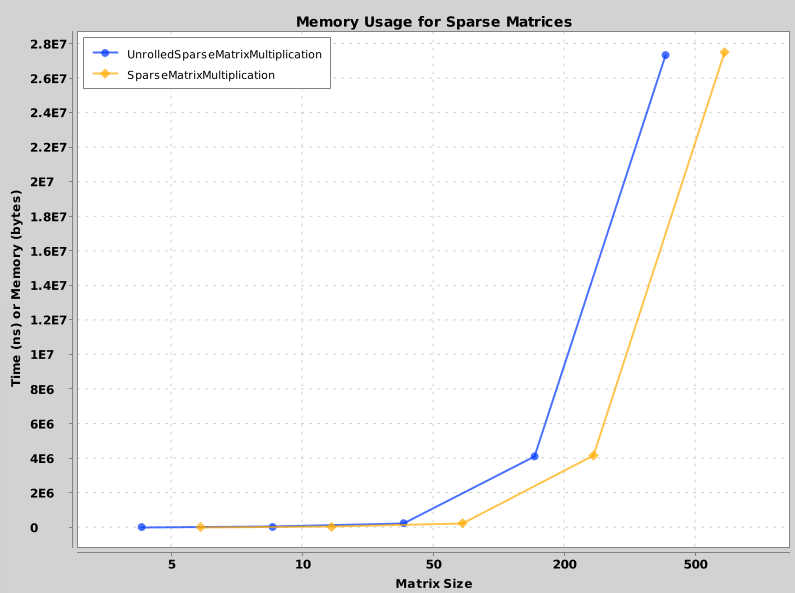
\includegraphics[width=\textwidth]{mem_sparse.png}
    \caption{Memory Usage for Sparse Matrices}
\end{figure}

\begin{figure}[h]
    \centering
    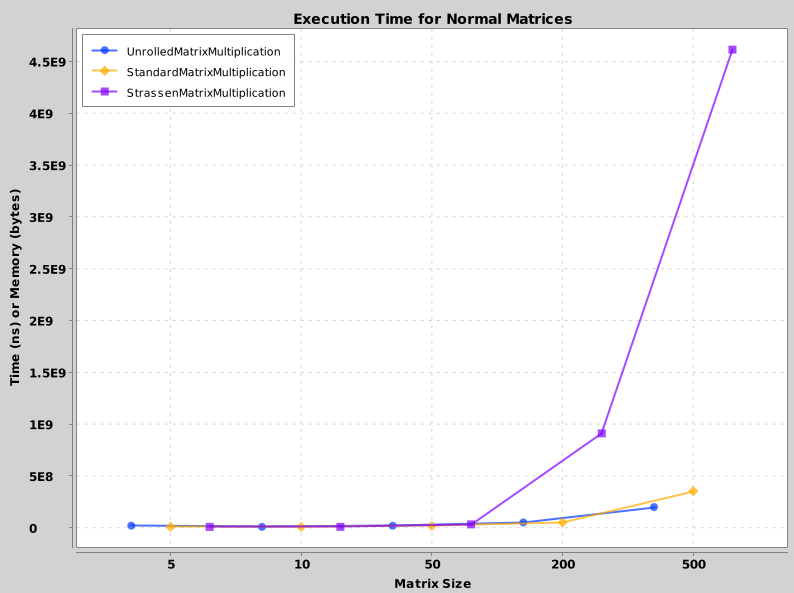
\includegraphics[width=\textwidth]{time_normal.png}
    \caption{Execution Time for Normal Matrices}
\end{figure}

\begin{figure}[h]
    \centering
    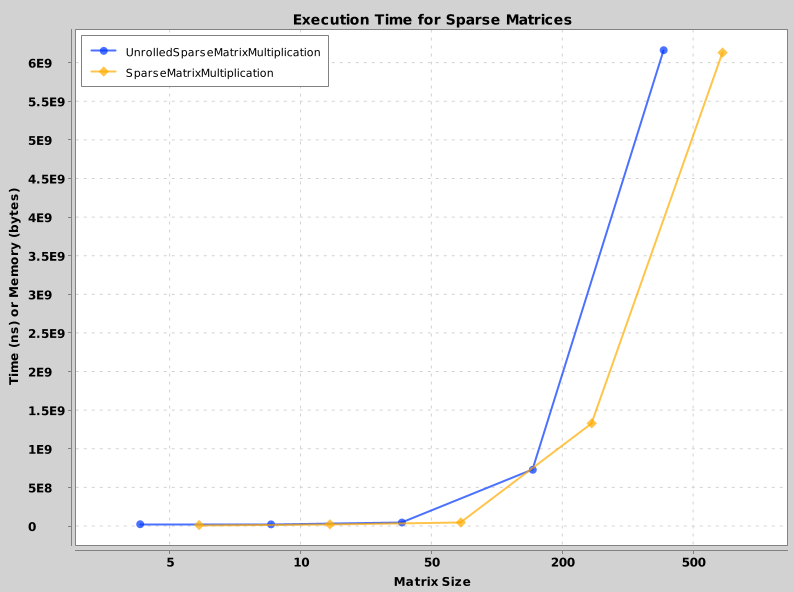
\includegraphics[width=\textwidth]{time_sparse.png}
    \caption{Execution Time for Sparse Matrices}
\end{figure}

\begin{figure}[h]
    \centering
    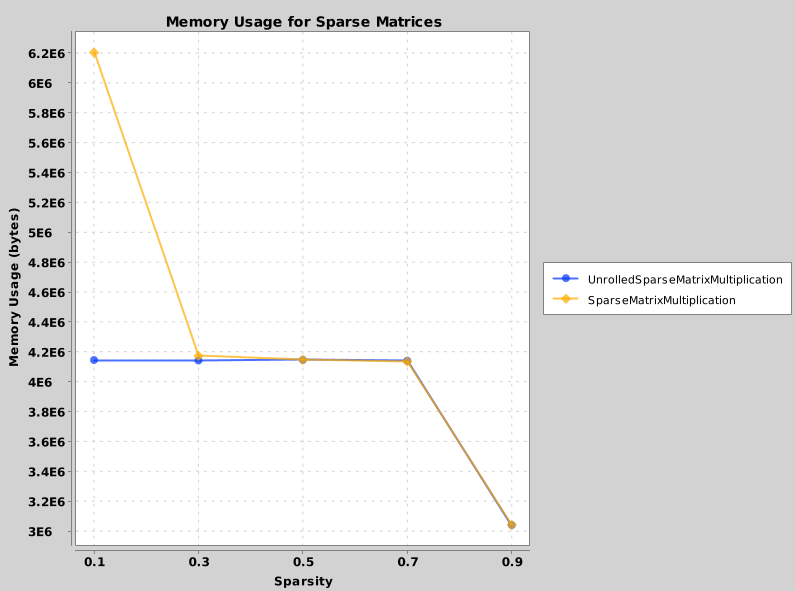
\includegraphics[width=\textwidth]{sparce_memory_comparison.png}
    \caption{Memory Comparison for Varying Sparse Matrices}
\end{figure}

\begin{figure}[h]
    \centering
    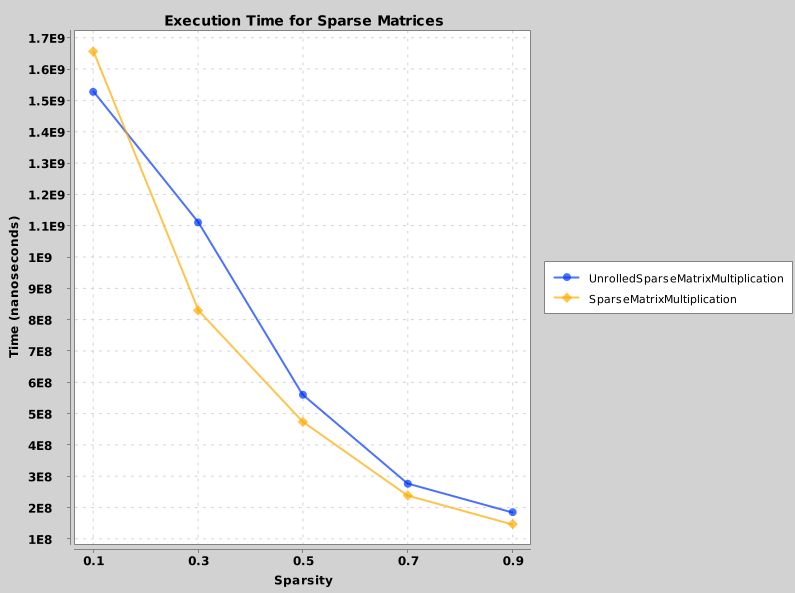
\includegraphics[width=\textwidth]{sparce_time_comparison.png}
    \caption{Time Comparison for Varying Sparse Matrices}
\end{figure}

\end{document}
